This section introduces the models and methods used in this work. Firstly, in \autoref{descr} we describe and explore the provided dataset. Secondly, in \autoref{baselines} we outline the baseline approaches used, and finally in \autoref{model} we describe our proposed RGNN architecture.

\subsection{Dataset Description} \label{descr}
The public Kaggle dataset\footnote{Kaggle dataset is available at \url{https://kaggle.com/c/cil-collaborative-filtering-2021/data}.} $X$ used in this work is composed of $|\mathcal{R}| = 1,176,952$ ratings ranging from $1$ to $5$. The ratings are given on $|\mathcal{I}| = 1000$ different items by $|\mathcal{U}| = 10000$ distinct users giving a sparsity of 11.77\% (quotient of total number of entries and observed entries). Compared to the Netflix Prize \citep{bennett2007netflix} and MovieLens \citep{harper2015movielens} datasets, we have a significantly denser data matrix which likely affects the choice of suitable algorithms \citep{lee2012comparative}.

Before proceeding further, we analyze whether matrix completion is information-theoretically possible. Note that most low-rank matrices have a logarithmic strong incoherence property in the order of $\mu^2 \in O(\log n)$ \cite{candestao}. Moreover, given the low sparsity of dataset $X$, we assume that $r = \text{rank}(X) \in O(1)$. By the Candés-Tao theorem \citep{candestao}, we need that the number of observed entries is $\smash{|\mathcal{R}| \in \Omega\left(|\mathcal{U}| \cdot \log^7\left(|\mathcal{U}|\right)\right)}$. Otherwise matrix completion is information-theoretically impossible.
Fortunately, according to the theorem the number of observed entries is sufficient in our case to enable matrix completion.

\subsection{Baselines} \label{baselines}
Our novel model is compared against the following baseline approaches used in collaborative filtering.
\begin{itemize}[leftmargin=0cm]
    \setlength\itemsep{0.6em}
    \item[]
    \textbf{SVD \citep{klema1980singular}:} Singular value decomposition (SVD) is a technique in which the data matrix (supposed all entries are observed) is decomposed into the product of two orthogonal matrices and a central diagonal one. The Eckart-Young theorem \cite{eckart1936approximation} is then used on this decomposition to obtain the best low-dimensional representation of the data. Since the user-item matrix is not complete in our case, the optimization of the recommendation system is done via learning representations of users and items through the alternating least squares (ALS) algorithm or gradient methods. In our implementation SVD uses stochastic gradient descent and is equivalent to probabilistic matrix factorization \citep{sala2007}.
    
    \item[]
    \textbf{SVD++ \citep{koren2008factorization}:} In contrast to SVD, SVD++ takes into account a form of implicit ratings. An implicit rating captures the information that some item is rated by some user. The concrete rating is disregarded in this implicit rating. Similarly to SVD, SGD is used to optimize the SVD++ objective.
    
    \item[]
    \textbf{NMF \citep{zhang2006learning, luo2014efficient}:} Non-negative matrix factorization (NMF) is the problem of approximately factorizing a given matrix by the product of two matrices with non-negative entries. In the context of collaborative filtering, learning such matrices loosely speaking means segmenting the items and users into categories such as genres and preferences. More specifically, the factorization can be interpreted as: (1) How much a user belongs to a certain category, and (2) by which category of users is a certain item preferred.
    
    \item[]\label{sec:slopeone}
    \textbf{SlopeOne \citep{lemire2005slope}:} This algorithm is arguably the simplest form of item-based collaborative filtering. SlopeOne predicts the non-observed rating of a user-item pair solely based on how another similar item has been rated. The prediction is made via a simple linear regressor of slope equal to $1$ (hence, the name) and a bias parameter which is learnt. The simplicity of this model increases computational efficiency. Additionally, overfitting induced by learning the slope vector is reduced.
    
    \item[]
    \textbf{NCF \citep{he2017neural}:} As opposed to canonical matrix factorization approaches, neural collaborative filtering (NCF) replaces the traditional sampling from the inner product between latent codes by a multi-layer perceptron (MLP). Contrary to the proposition in the NCF paper, the generalized matrix factorization (GMF) is omitted in our implementation since the standalone MLP outperformed the combination of the MLP and GMF on our dataset.
    
    \item[]
    \textbf{GNN \citep{wang2019neural}:} The main idea of a graph neural network (GNN) for collaborative filtering consists of representing users and items as nodes of a bipartite graph. Edges between the two partitions of the graph are weighed by a (normalized) rating given by a user for the item. The GNN architecture progressively aggregates and propagates neighborhood latent information generating embeddings of the users and items. Ratings are predicted using a single linear layer. A more detailed description of the GNN and our implementation is provided in \autoref{mapping_and_embedding}.
\end{itemize}


\subsection{Reinforced Graph Neural Networks} \label{model}
We propose the novel architecture: reinforced graph neural networks (RGNNs). The architecture consists of stacking together a graph neural network (as inspired by \citet{wang2019neural, wu2021graph}) with a feed-forward network and adding reinforcements. The graph neural network is the GNN \citep{wang2019neural} and the feed-forward network is the NCF \citep{he2017neural} as described in \autoref{baselines}. The GNN learns the embeddings of users and items, and these embeddings are then pushed through the feed-forward network of the NCF to make reliable and accurate rating predictions. Additionally, we have derived a similar concept to reliabilities introduced by \citet{reliability} which we denote reinforcements (see \autoref{reinforcements}). These concepts allow us to construct a novel architecture obtaining the best of both worlds: (1) The strength of graph-extracted embeddings, and (2) the generalization power of deep learning architectures.

\subsubsection{Theoretical description}
As depicted in \autoref{fig: model}, the RGNN model consists of four phases. The phases can be described disjointly and are: (1) The mapping phase, (2) the embedding phase, (3) the prediction phase, and (4) the combination phase. Note that the phases (1) - (3), described in \autoref{alg:gnn_ncf}, are called GNN + NCF in the remainder of this work. The combination phase (4) predicts a rating from a given output of the GNN + NCF and the corresponding reinforcement. Training the RGNN is done using standard backpropagation minimizing the mean squared error loss.

\begin{figure*}
    \centering
    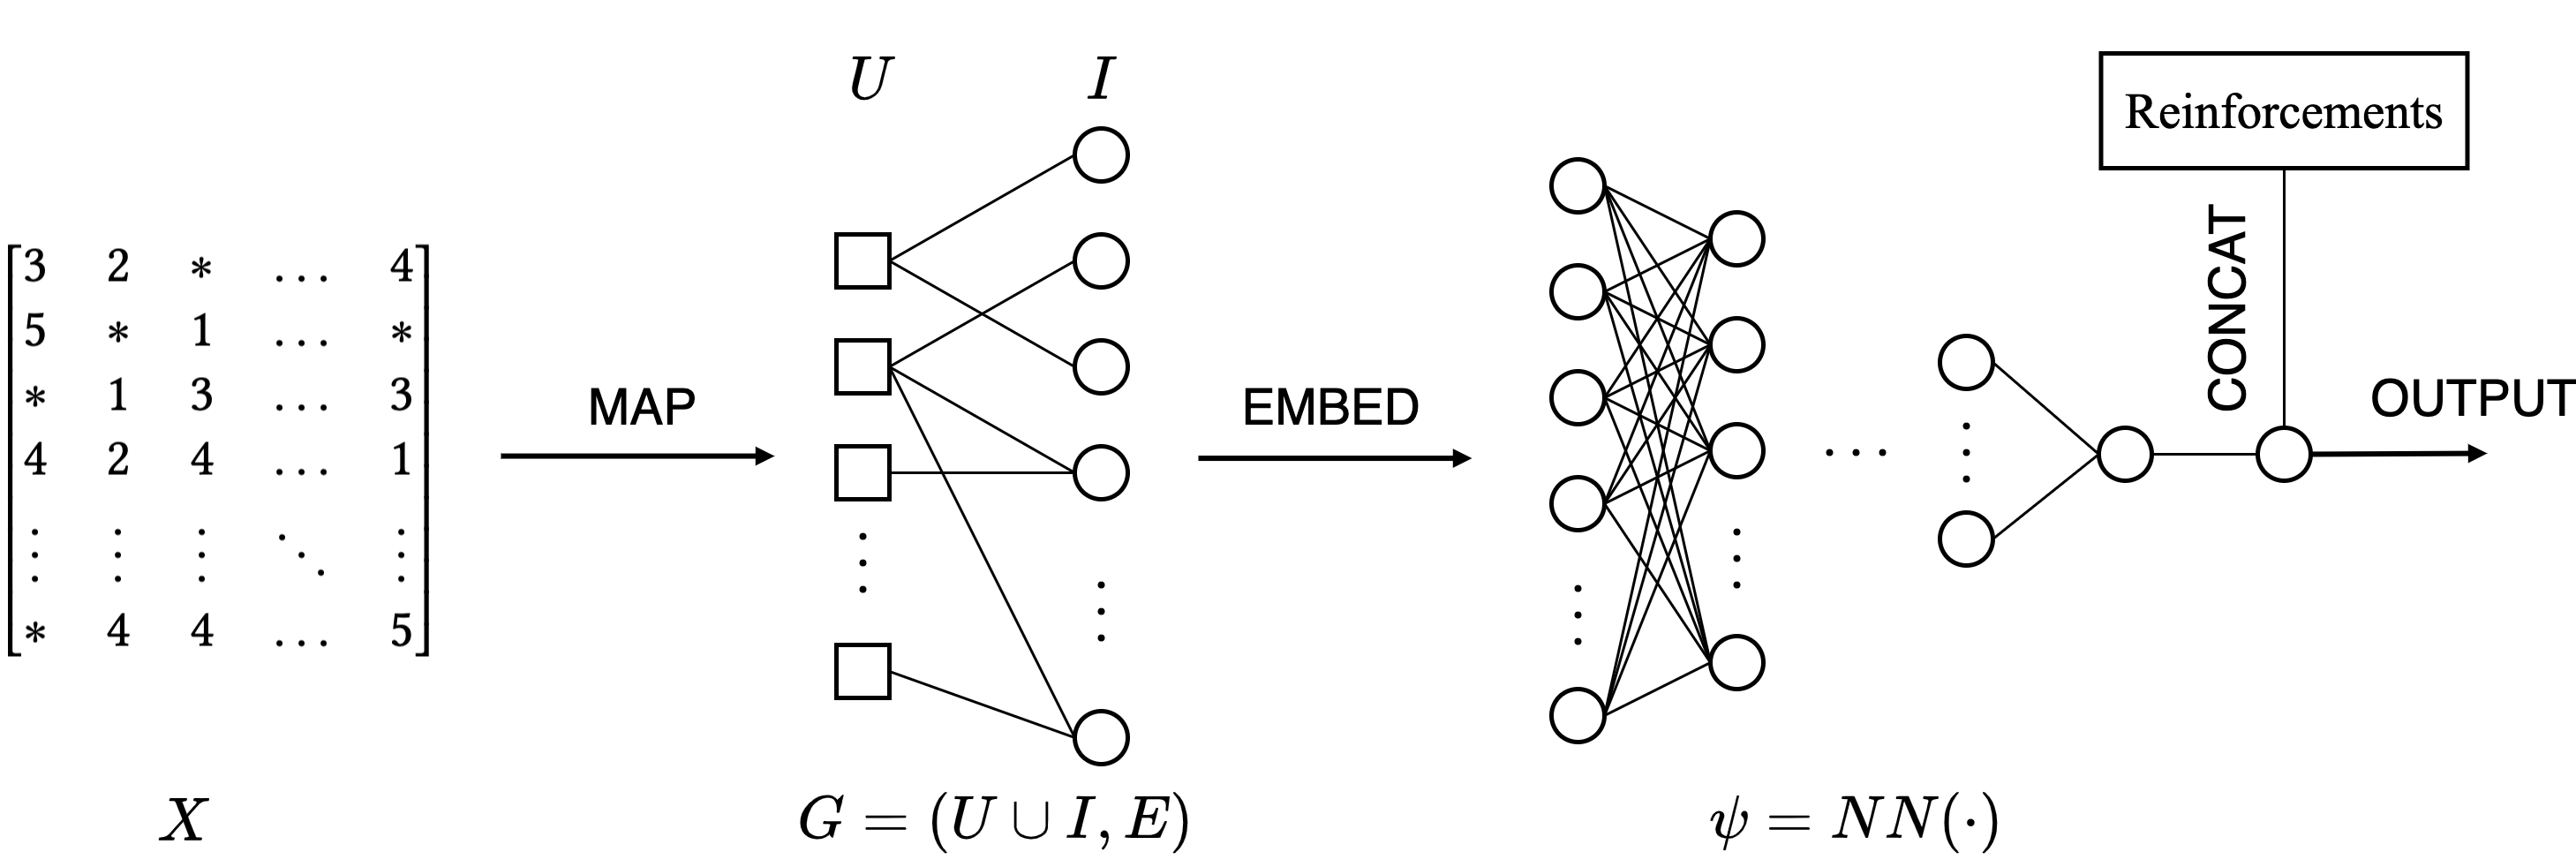
\includegraphics[width=0.9\textwidth]{figures/rgnn_architecture.png}
    \caption{RGNN architecture. (left) Sparse user-item rating data matrix. (center) Bipartite graph representation of the data. (right) Feed-forward neural network that takes the graph-learnt user and item embeddings as well as the reinforcements as input and outputs the rating predictions.}
    \label{fig: model}
\end{figure*}

\subsubsection{Mapping and Embedding}\label{mapping_and_embedding} The dataset $X$ represents the sparse adjacency matrix of the bipartite graph $G = (U \cup I, E)$, where $U$ denotes the partition of user nodes, $I$ the partition of items, and $E$ the set of edges weighted by the observed user-item ratings (line 1 in \autoref{alg:gnn_ncf}). For node $v \in U \cup I$, let $\textbf{m}^{\ell}$ represent the aggregated neighbor information of node $v$ at layer $\ell$, $\textbf{e}^{\ell}_v$ its hidden state (or embedding) at layer $\ell$, and $\textbf{N}_v$ its neighborhood. During the embedding phase, the GNN + NCF algorithm simulates the aggregation of information in the $L$-hop neighborhood of node $v$. This helps extracting higher-order relations between users and items.

The information about nodes in the $L$-hop neighborhood of some node $v \in U \cup I$ is made iteratively and is shown in lines 4 - 7 in \autoref{alg:gnn_ncf}. In particular, at each iteration the aggregated neighbor information $\textbf{m}^{\ell}_v$ of node $v$ is computed by taking the sum over the neighbor information for each neighbor $i \in \textbf{N}_v$ normalized by a discount factor of $\smash{{(\left|\textbf{N}_v\right|\left|\textbf{N}_i\right|})^{-\frac{1}{2}}}$. The discount factor accounts for the decay of the influence of $\ell$-hop neighbors. The neighbor information for a node pair ($v$, $i$) is calculated as a weighted combination of the embedding $\textbf{e}^{\ell}_v$ of node $v$ and the element-wise composition, denoted by $\odot$, of the embedding $\textbf{e}^{\ell}_v$ of $v$ and the embedding $\textbf{e}^{\ell}_i$ of the neighbor $i$. Using the aggregated neighbor information of node $v$ for the $\ell$-hop neighborhood and the $\ell$-hop embedding, we compute the $(\ell + 1)$-hop embedding. This computation takes the sum of the weighted $\ell$-hop embedding and the aggregated neighbor information $\textbf{m}^{\ell}_v$. Further, the Rectified Linear Unit (ReLU) activation function is applied to obtain the $(\ell + 1)$-hop embedding $\textbf{e}^{\ell + 1}_v$. Note that $\textbf{W}_1$ and $\textbf{W}_2$ are the set of parameters that respectively weigh how much the current embedding is influenced by the original features and to what extent the later hops information affects the embedding. An embedding for a node $v$ is then the concatenation of the $\ell$-hop embeddings $\textbf{e}^{\ell}_v$ (line 8 in \autoref{alg:gnn_ncf}).

\subsubsection{Prediction} For a given user-item pair ($u$, $i$), the input to the prediction phase is the embeddings of the user $\textbf{e}^{*}_u$ and item $\textbf{e}^{*}_i$. The output is then computed by the feed-forward network denoted by $\textbf{NN}$ in \autoref{alg:gnn_ncf}. In particular, the feed-forward network is the same as the one used for the NCF baseline (see \autoref{baselines}).

\begin{algorithm}
    \caption{GNN + NCF} \label{alg:gnn_ncf}
    
    \SetAlgoLined
    \DontPrintSemicolon
    \Init{
        Map data matrix $X$ to graph $G = (U \cup I, E)$ \;
    }
    
    \For{$v \in U \cup I$}{
        \For{$\ell \in [L-1]$}{
            $\textbf{m}^{\ell}_v = \sum_{i \in \textbf{N}_v}{\frac{1}{\sqrt{\left|\textbf{N}_v\right|\left|\textbf{N}_i\right|}}\left(\textbf{W}^{\ell}_1\textbf{e}^{\ell}_i + \textbf{W}^{\ell}_2\left(\textbf{e}^{\ell}_i \odot \textbf{e}^{\ell}_v\right)\right)}$ \;
            
            $\textbf{e}^{\ell + 1}_v = \text{ReLU}\left(\textbf{W}^{\ell}_1\textbf{e}^{\ell}_v + \textbf{m}^{\ell}_v\right)$ \;
        }
        
        Concatenate the embeddings: $\textbf{e}^{*}_v = \textbf{e}^{1}_v \oplus \dots \oplus \textbf{e}^{L}_v$ \;
    }
        
    Predict Rating: $\hat{y}(u,i) = \textbf{NN}\left( \textbf{e}^{*}_u\oplus\textbf{e}^{*}_i\right)$ for user-item pair ($u$, $i$) \;
\end{algorithm}

\subsubsection{Reinforcements}\label{reinforcements} Since the input to the GNN + NCF model simply consists of user-item pairs, we aim at providing additional information to the network. Inspired by the approach of \citet{reliability}, where the authors use the prediction accuracy of a model as an additional input to the final model, we introduce reinforcements. Reinforcements consists of predictions from different baseline models. The reinforcements are then fed into a single linear layer together with the output of the GNN + NCF to yield the final predictions of our RGNN. An example of a reinforcement type is the SVD baseline, where the reinforcements for users $u \in U$ and items $i \in I$ are computed using SVD. Then, when introducing the reinforcement for a given user-item pair in the RGNN, the reinforcement intuitively holds the information on how good the SVD baseline prediction is compared to the prediction of the GNN + NCF. This concept is easily extended to different reinforcement types. In particular, our model supports reinforcements from the SVD, SVD++, NMF, and SlopeOne baselines. Additionally, multiple reinforcements can be used simultaneously. However, as we will see in the experimental evaluation of our model in \autoref{sec:results}, the best performance is obtained with a single reinforcement, namely the SlopeOne reinforcement.

\subsubsection{Network Architecture} The RGNN uses two different neural network architectures used for the embedding and predictions. This section provides a brief description of both architectures and the layers used.

The embedding architecture is the GNN baseline and embeds a user or item using three embedding propagation layers. As mentioned in section~\ref{mapping_and_embedding}, these layers accumulate the information in the three-hop neighborhood of the current node in the bipartite graph. The resulting embedding of a user or item is then of size $3 \times 64$.

The prediction architecture is the feed-forward network of the NCF baseline taking as an input the embedding of one user and one item. The network has the following layers: \emph{Dropout, Linear (384), ReLU, Dropout, Linear (64), ReLU, Dropout, Linear (32), ReLU, Linear (16), ReLU, Linear (8), ReLU, Output (1)}. The output of the network is then combined using the reinforcements in a final linear layer. Note that as with the NCF architecture, the prediction architecture contains dropout nodes. However, the optimal dropout rate found during hyperparameter tuning was $0.0$. This supports the findings of the paper introducing graph neural networks \citep{wang2019neural}.

\subsubsection{Ensemble learning}
We improve predictions by utilizing ensembles of our RGNN model with a simple model averaging method for generating the final predictions. We obtained best results using 12 models with SlopeOne reinforcements and different random seeds. We further tried averaging predictions of RGNNs with different reinforcement combinations, however, this showed inferior performance compared to the SlopeOne reinforcements with different random seeds.